\documentclass[12pt]{article}
\usepackage{geometry}                % See geometry.pdf to learn the layout options. There are lots.
\geometry{letterpaper}                   % ... or a4paper or a5paper or ... 
\usepackage{graphicx}
\usepackage{amssymb}
\usepackage{amsthm}
\usepackage{epstopdf}
\usepackage[utf8]{inputenc}
\usepackage[usenames,dvipsnames]{color}
\usepackage[table]{xcolor}
\usepackage{hyperref}
\usepackage[utf8]{inputenc}
\usepackage[T1]{fontenc}
\usepackage{lmodern}
\usepackage{caption}
\usepackage{floatrow}%
\DeclareGraphicsRule{.tif}{png}{.png}{`convert #1 `dirname #1`/`basename #1 .tif`.png}

\theoremstyle{definition}
\newtheorem{example}{Example}


\newcommand{\projectname}{Allround Manager}
\newcommand{\productname}{Allround Manager}
\newcommand{\projectleader}{Christian Bachl}
\newcommand{\documentstatus}{In process}
%\newcommand{\documentstatus}{Submitted}
%\newcommand{\documentstatus}{Released}
\newcommand{\version}{V. 1.0}

\begin{document}
\begin{titlepage}
\begin{flushright}
%\includegraphics[scale=.5]{htlleondinglogo.png}\\
\end{flushright}

\vspace{10em}

\begin{center}
{\Huge System Specification} \\[3em]
{\LARGE \productname} \\[3em]
\end{center}

\begin{flushleft}
\begin{tabular}{|l|l|}
\hline
Project Name & \projectname \\ \hline
Project Leader & \projectleader \\ \hline
Document state & \documentstatus \\ \hline
Version & \version \\ \hline
\end{tabular}
\end{flushleft}

\end{titlepage}
\section*{Revisions}
\begin{tabular}{|l|l|l|}
\hline
\cellcolor[gray]{0.5}\textcolor{white}{Date} & \cellcolor[gray]{0.5}\textcolor{white}{Author} & \cellcolor[gray]{0.5}\textcolor{white}{Change} \\ \hline
November 29, 2018&C. Christian/Jusic version \\ \hline
\end{tabular}
\pagebreak

\tableofcontents
\pagebreak

\section{Initial Situation and Goal}

\subsection{Initial Situation}
Organizing an event involves a lot of organizational steps for the event leader. A non-exhaustive list of tasks could be
\begin{itemize}
\item When the event involves some trip a generally accepted destination has to be aligned
\item Send invitations to all participants
\item Keeping track of registrations or de-registration of participants
\item Gathering information about the participants like home addresses, passport numbers, etc.
\item Provisioning of information about the event for the participants, like the aim of the event, agenda, other participants, etc.
\item bills of outstanding services like a prepayment for an event.
\end{itemize}

Currently, a wide variety of tools has to be used to accomplish the above-mentioned tasks.
\begin{itemize}
\item Most of the communication is done via WhatsApp or similar social media apps.
\item Lists of participants, their status, etc. are organized via spreadsheets
\item Outstanding bills must be paid with a payment slip or in cash.
\end{itemize}


The combination of different tools and a very decentralized way of organization makes it hard for the event organizer to stay on top of the things. More often than not these events struggle with late minute change or an announcement.  This could be:
\begin{itemize}
\item meeting point of the event/journey.
\item A date where the event takes place.
\end{itemize}


Doing these things may cause some troubles for the event organizer, like:

\begin{itemize}
\item when you have a lot of participants you may forget somebody
\item When billing, for example, participants want to pay only from the location where they have entered.
\item the leader must be every time available like: user wants to de-register or want to know many participants take part in the event.
\item getting spammed by registrations in WhatsApp.  
\end{itemize}


\subsubsection{Application Domain}



\subsubsection{Glossary}

\subsubsection{Model of the Application Domain}

\subsection{Goal Definition}
The main goal is to create a software to speed up and simplify the process of organizing an event. We especially want to make it possible for people who don't have the opportunity to afford expansive software or an event manager.
\pagebreak

\section{Functional Requirements}

\subsection{Use Case Join Event}

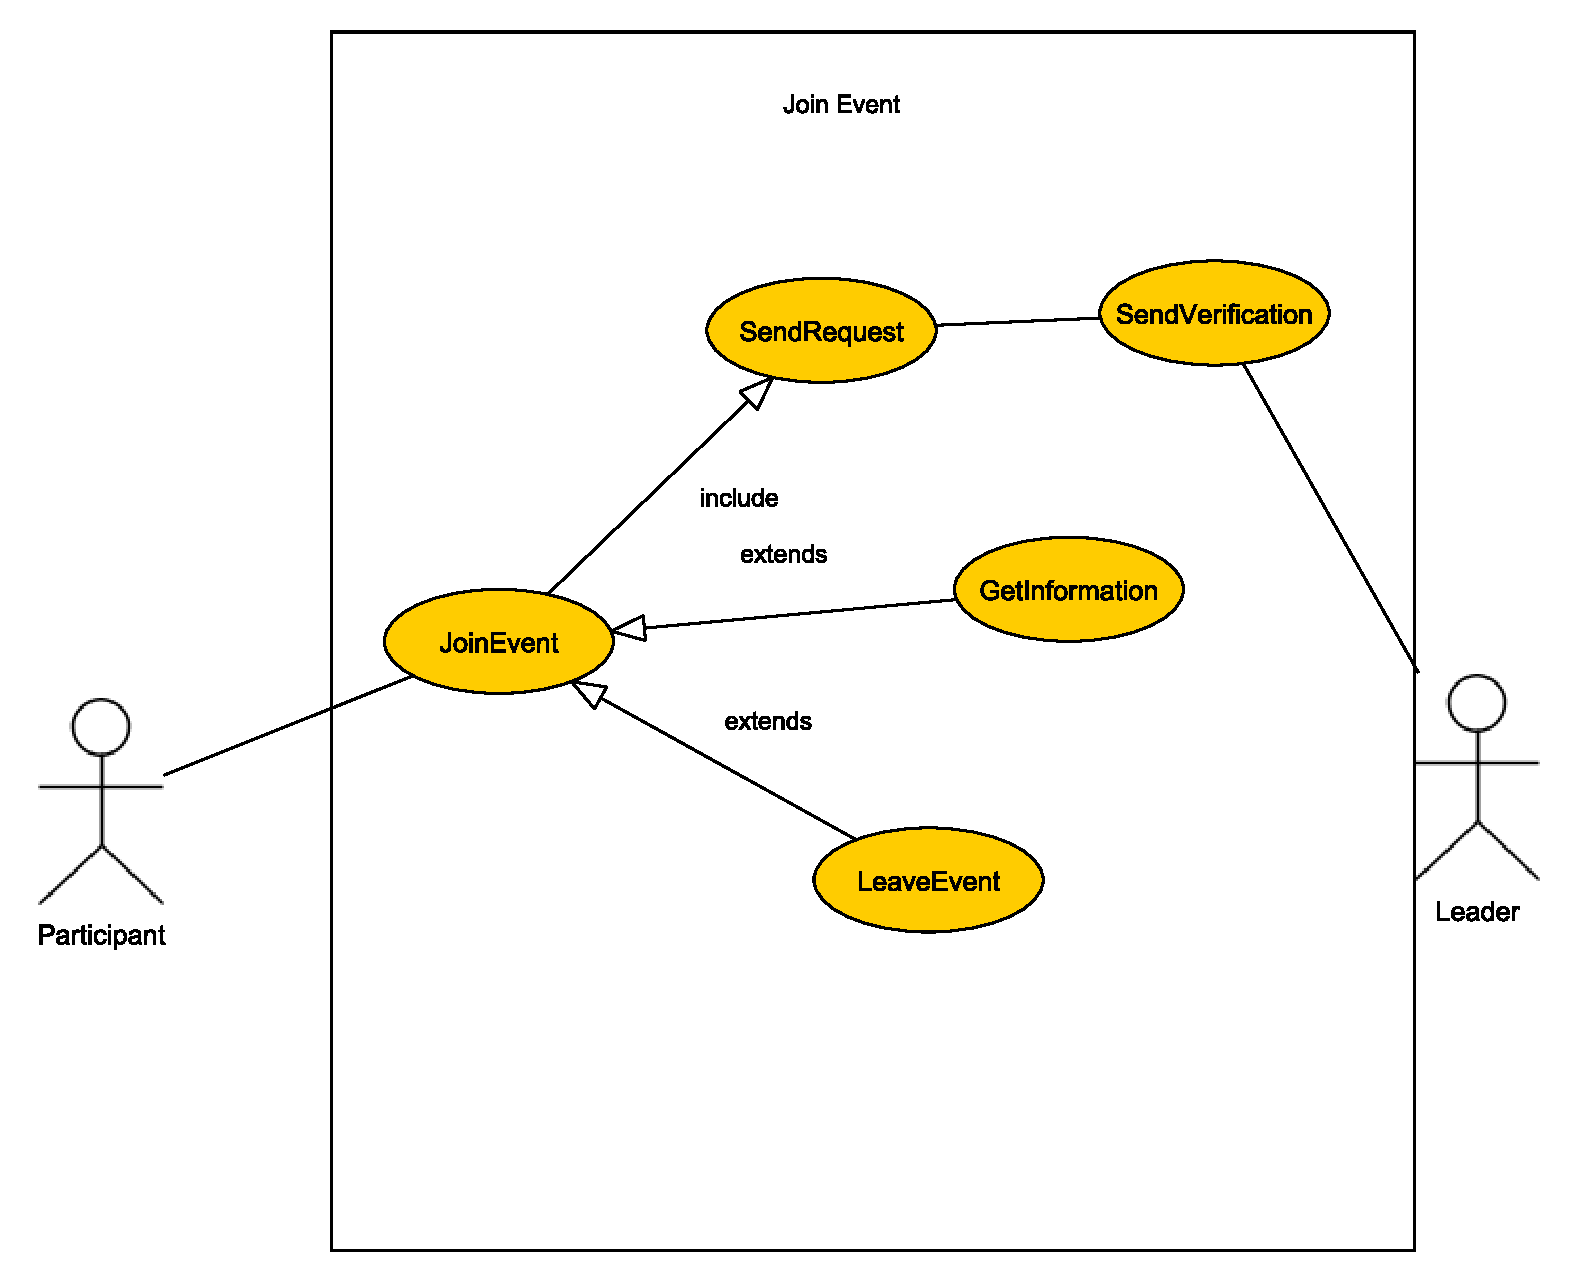
\includegraphics[scale=.5]{Usecase/JoinEvent.pdf}

\subsubsection{Use Case Details}

If the user wants to join an event, he must first be accepted by the leader. You get a verification from the leader. Of course the user can also leave the event. If he doesn't want to leave the event and really wants to participate, he will get all necessary information about the event from the leader.

\subsubsection{Characteristic Information}

\begin{tabular}{|l|l|}
\hline
Goal & To add a user to the participant list and add a entry on his event list \\ \hline
Precondition &  The event is not full and the Leader accept his join request\\ \hline
Involved User &  The user who want to join the event and the leader for accepting him to join the event\\ \hline

\end{tabular}


\subsection{Use Case Join Group}

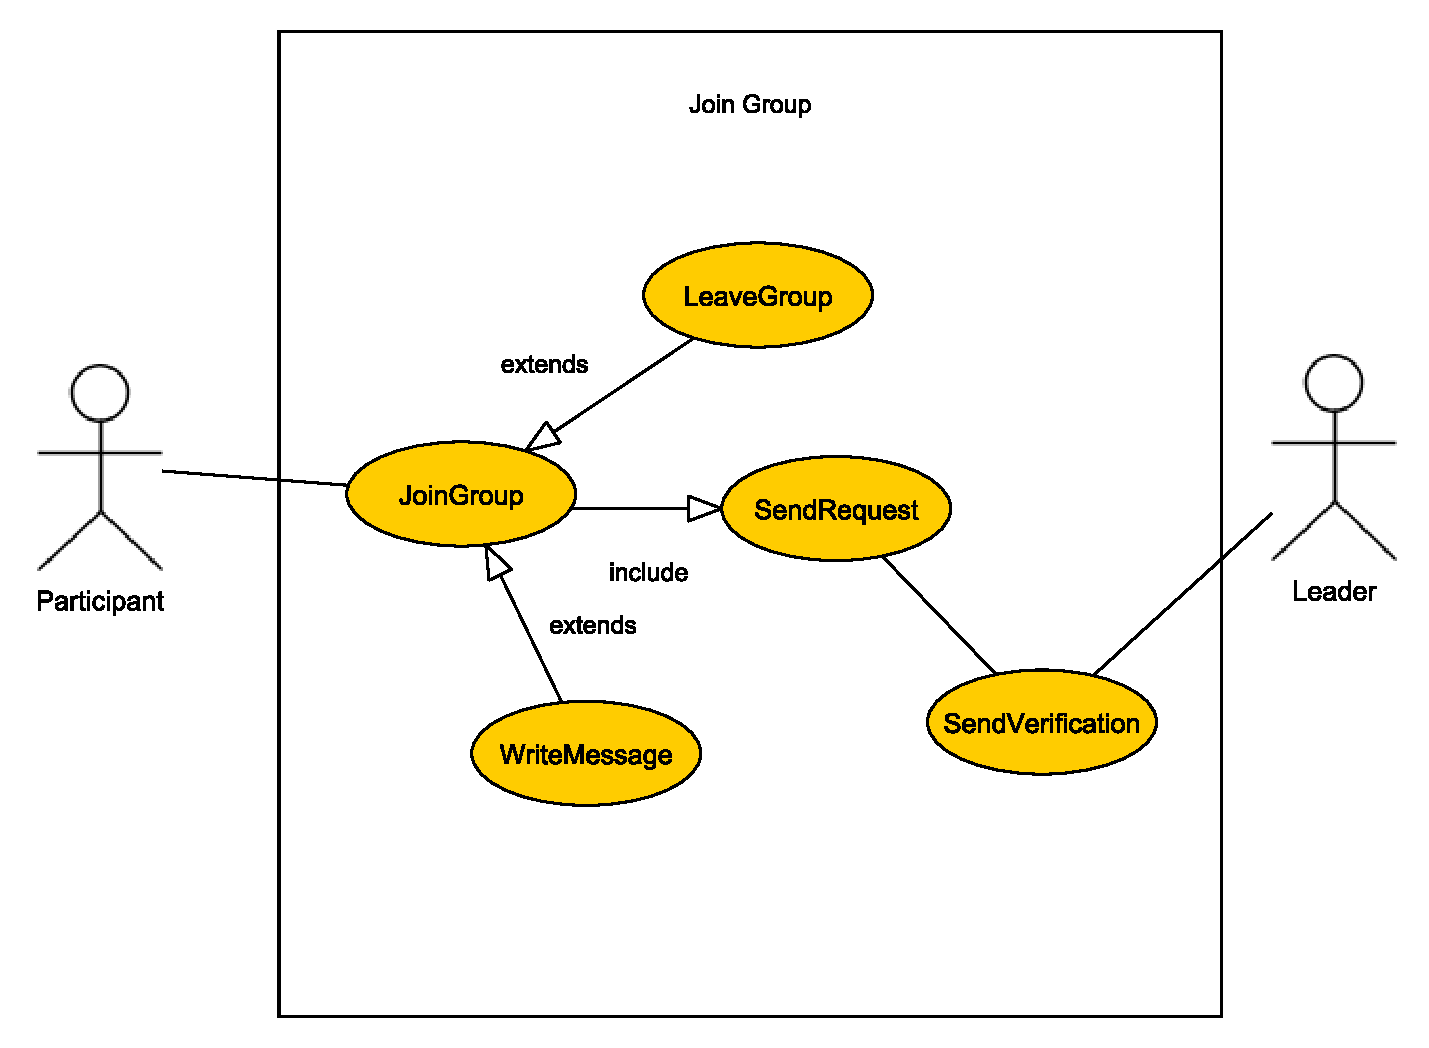
\includegraphics[scale=.5]{Usecase/JoinGroup.pdf}

\subsubsection{Use Case Details}

If the user wants to join a group, he must first be accepted by the leader. He also receives a confirmation from the leader. If the user is in a group, he can send messages and of course leave the group.
\subsubsection{Characteristic Information}

\begin{tabular}{|l|l|}
\hline
Goal & To add a user to the participant list and add a entry on his event list \\ \hline
Precondition &  The event is not full and the Leader accept his join request\\ \hline
Involved User &  The user who want to join the event and the leader for accepting him to join the event\\ \hline

\end{tabular}


\subsection{Use Case Create Event}

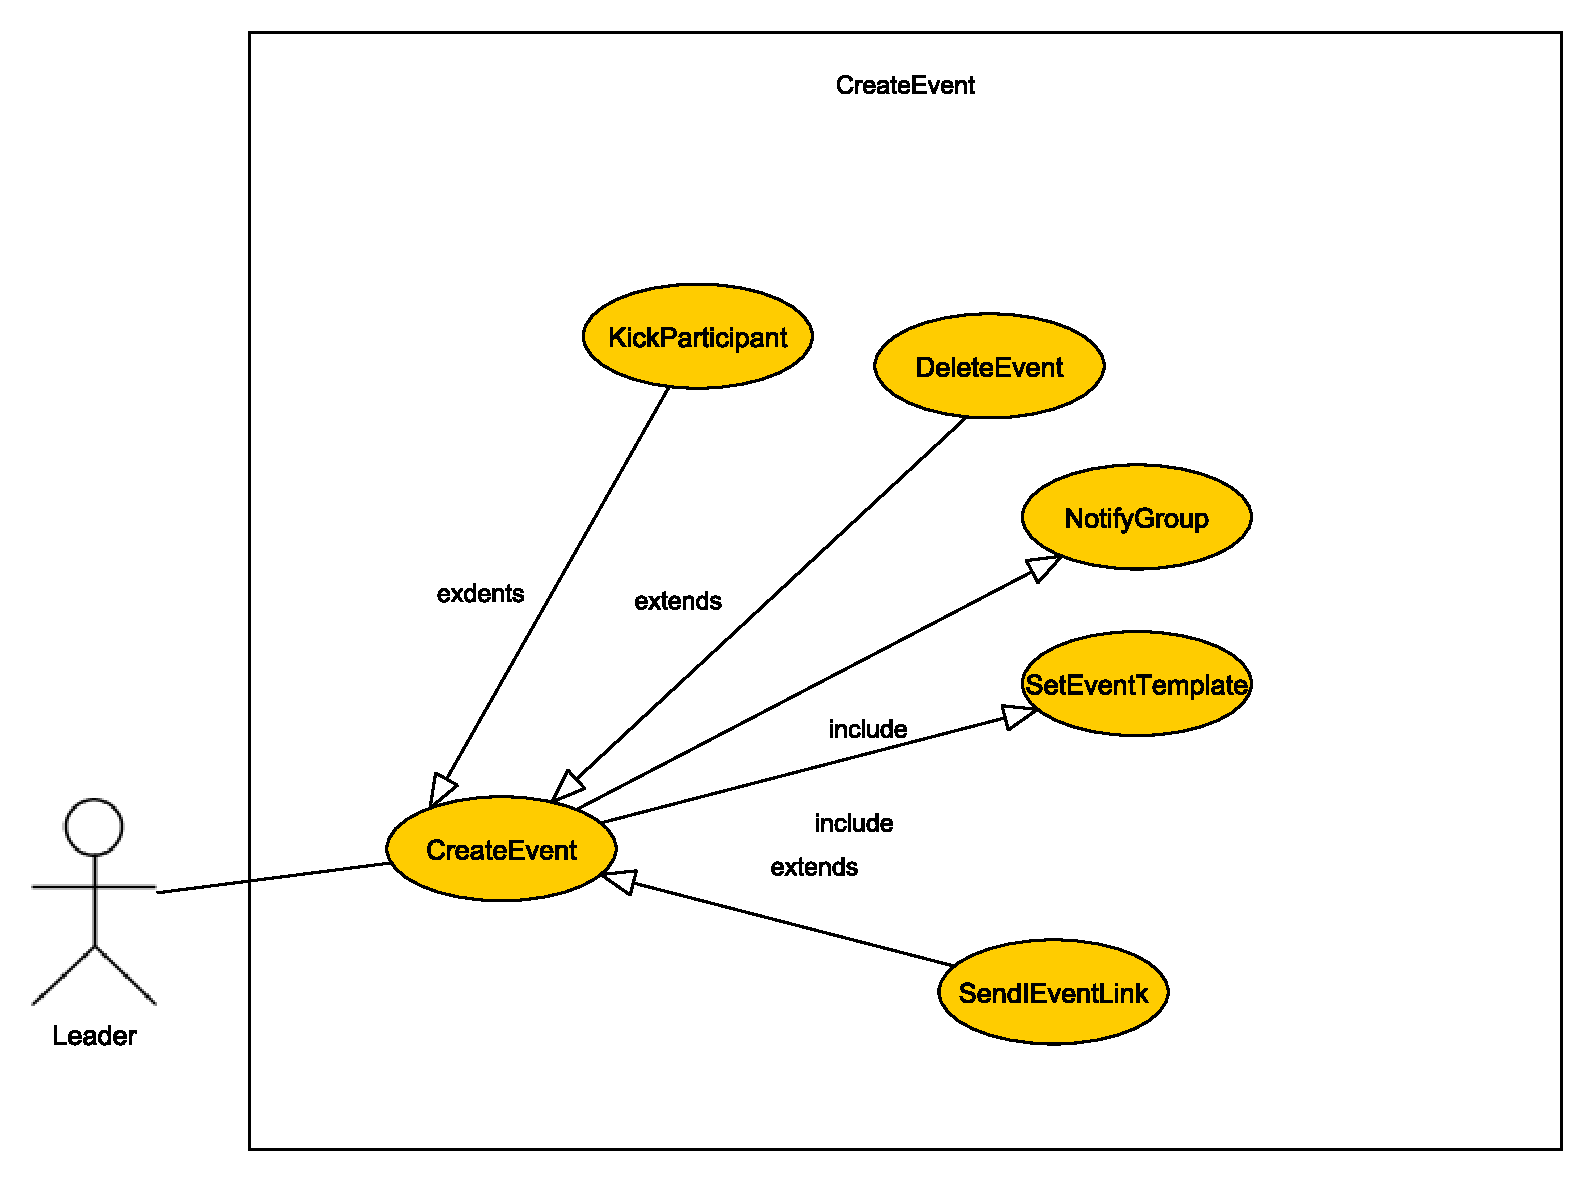
\includegraphics[scale=.5]{Usecase/CreateEvent.pdf}

\subsubsection{Use Case Details}

The leader creates an event. He must select a template or create one himself. If the leader is in a group with other participants, they get a notification. the leader can send the link to the event so that others can participate. He can also kick out the participants or delete the event.

\subsubsection{Characteristic Information}

\begin{tabular}{|l|l|}
\hline
Goal & To add a user to the participant list and add a entry on his event list \\ \hline
Precondition &  The event is not full and the Leader accept his join request\\ \hline
Involved User &  The user who want to join the event and the leader for accepting him to join the event\\ \hline

\end{tabular}

\subsection{Use Case Create Group}

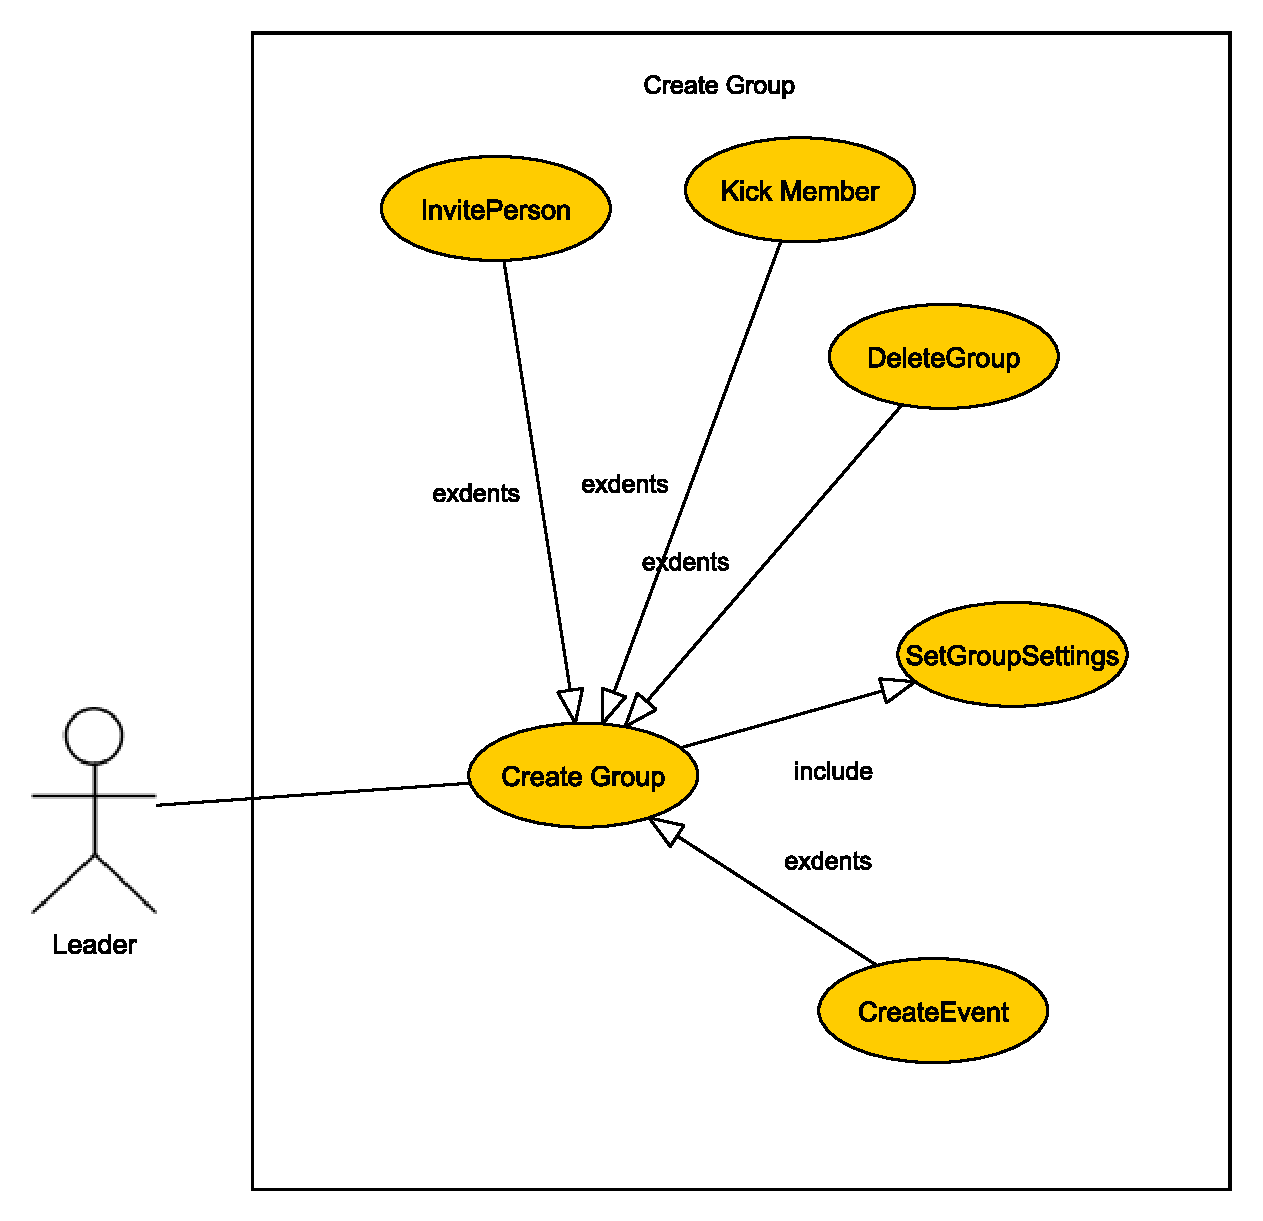
\includegraphics[scale=.5]{Usecase/CreateGroup.pdf}

\subsubsection{Use Case Details}

The leader creates an event. He must select a template or create one himself. If the leader is in a group with other participants, they get a notification. the leader can send the link to the event so that others can participate. He can also kick out the participants or delete the event.

\subsubsection{Characteristic Information}

\begin{tabular}{|l|l|}
\hline
Goal & To add a user to the participant list and add a entry on his event list \\ \hline
Precondition &  The event is not full and the Leader accept his join request\\ \hline
Involved User &  The user who want to join the event and the leader for accepting him to join the event\\ \hline

\end{tabular}


\pagebreak

\section{Non-functional Requirements}

\begin{flushleft}
  \begin{tabular}{|l|l|}
  \hline
  ID & NFR001\\ \hline
  Name & Data volume \\ \hline
  Type &  EFFIC\\ \hline
  Description & The data usage should be under 75 mb per month \\
  & given that not a lot of pictures are up/downloaded. \\
  & Assuming 8 Mbit/s download 2 Mbit/s upload. \\ \hline
  \end{tabular}
\end{flushleft}

\vspace*{1 cm}

\begin{flushleft}
  \begin{tabular}{|l|l|}
  \hline
  ID &  NFR002\\ \hline
  Name & Start time \\ \hline
  Type &  EFFIC\\ \hline
  Description & The synchronisation of the user configuration and \\
  & the database should not take longer than 5 seconds. \\ 
  & Assuming 8 Mbit/s download 2 Mbit/s upload. \\ \hline
  \end{tabular}
\end{flushleft}

\vspace*{1 cm}

\begin{flushleft}
  \begin{tabular}{|l|l|}
  \hline
  ID &  NFR003\\ \hline
  Name & Group \\ \hline
  Type &  EFFIC\\ \hline
  Description & Changes to the group should not take \\
  & longer than 1 second to upload. \\ 
  & Assuming 8 Mbit/s download 2 Mbit/s upload. \\ \hline
  \end{tabular}
\end{flushleft}

\vspace*{1 cm}

\begin{flushleft}
  \begin{tabular}{|l|l|}
  \hline
  ID &  NFR003\\ \hline
  Name & Accessibility \\ \hline
  Type &  SEC \\ \hline
  Description & The only data we need to protect from \\
  & unauthorized access are the users password and e-mail address. \\ \hline
  \end{tabular}
\end{flushleft}


\pagebreak

\section{Quantity Structure}
Every user has a nickname, password and e-mail. All configuration from every user concerning hometown, address and age will be saved independetly for every event. An event has its
own information about the date, when the event takes place, the number of participants, which participants are included. Those informations can be also seen by every member. A new user with the default configuration will use about 90 records. Considering the amount of data we chose to save the user data in a database. 

\pagebreak



\section{System Architecture and Interfaces}
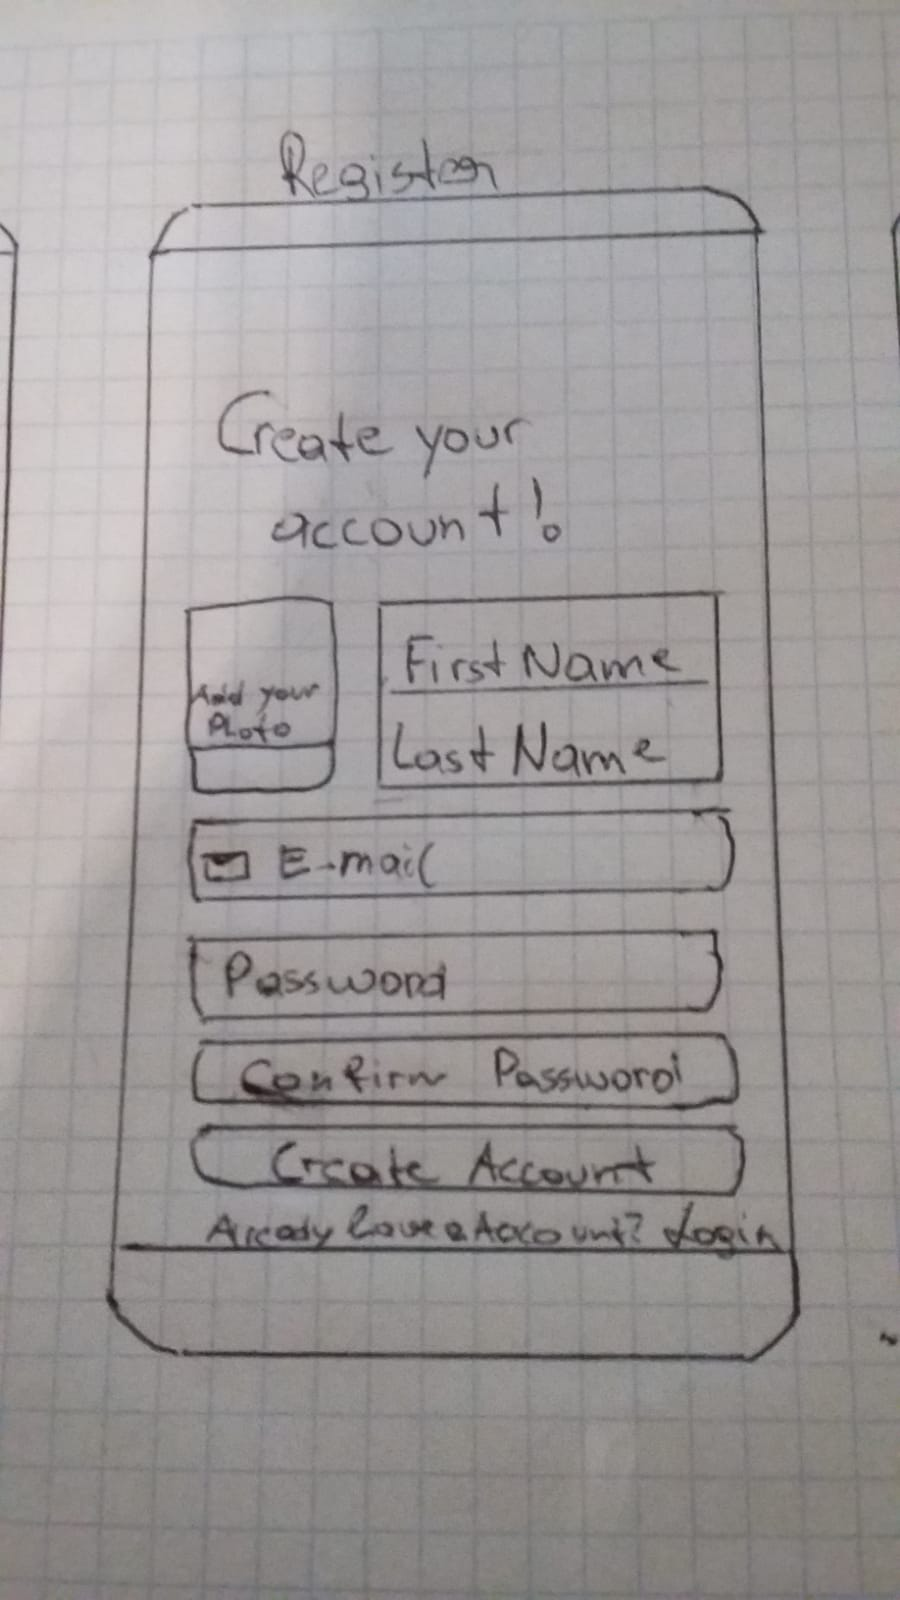
\includegraphics[scale=.2]{Gui/register.jpeg}


\pagebreak

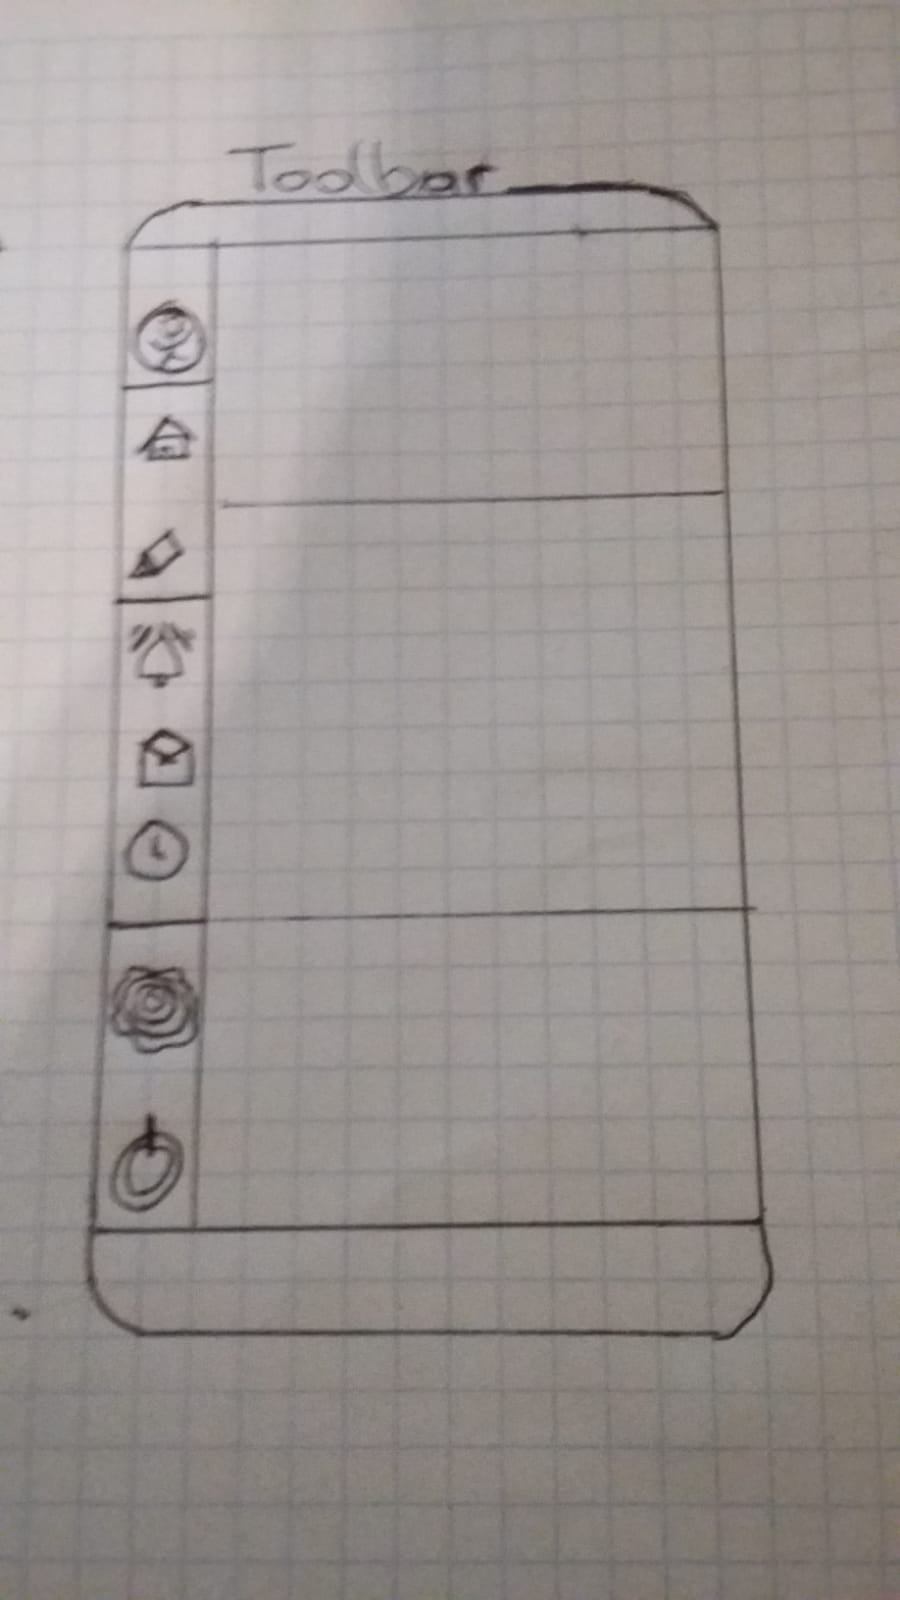
\includegraphics[scale=.2]{Gui/toolbar.jpeg} 
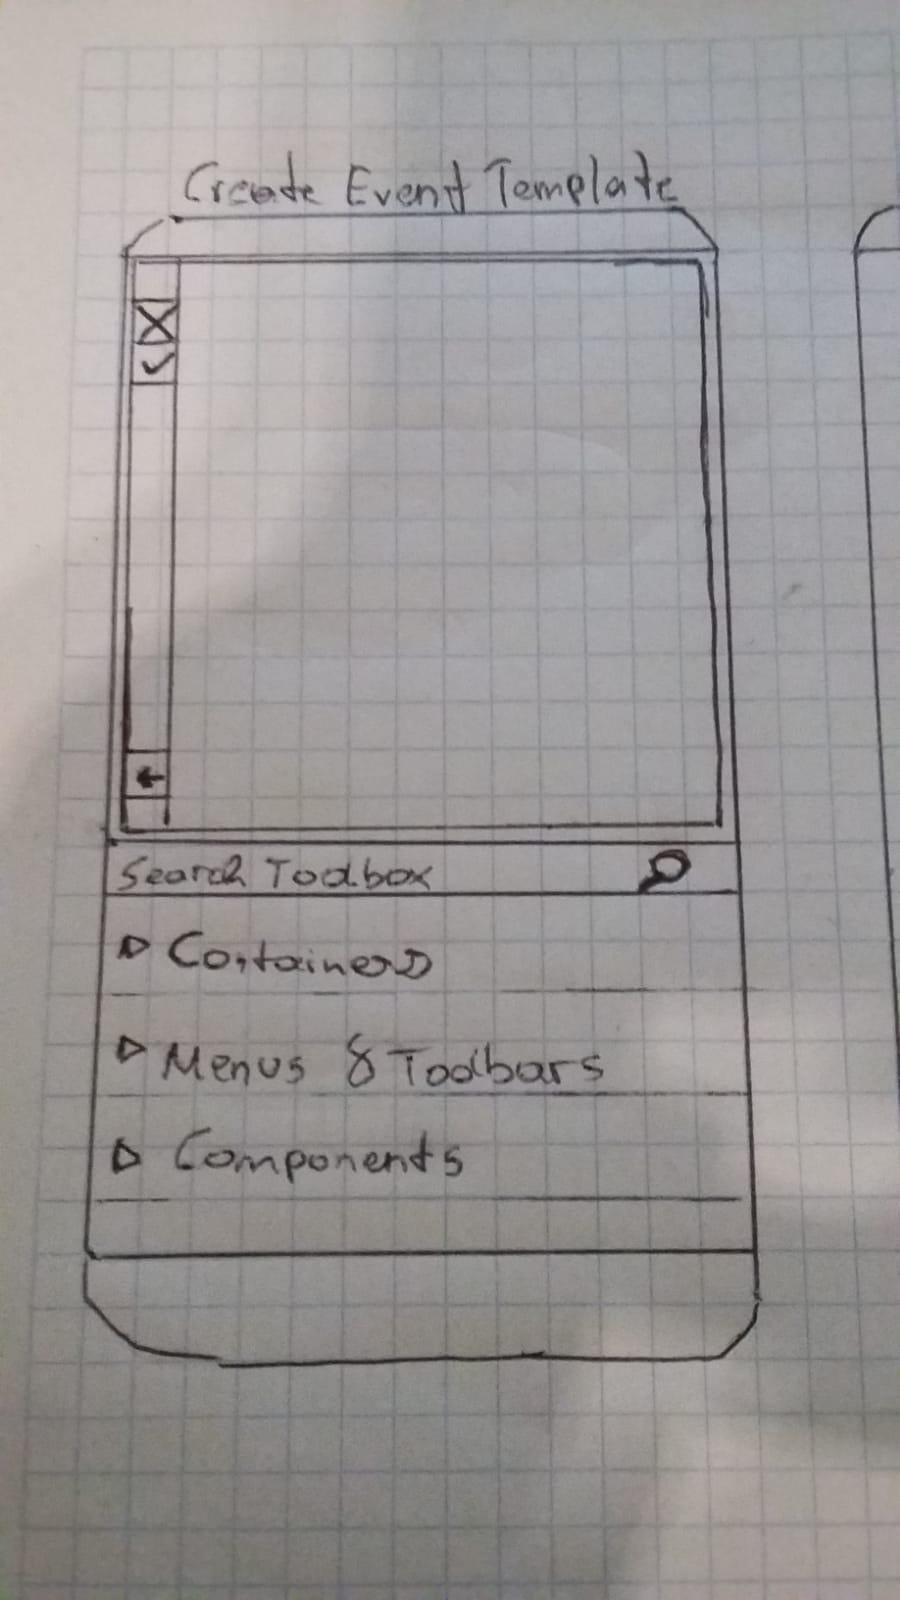
\includegraphics[scale=.2]{Gui/create_event.jpeg} \\
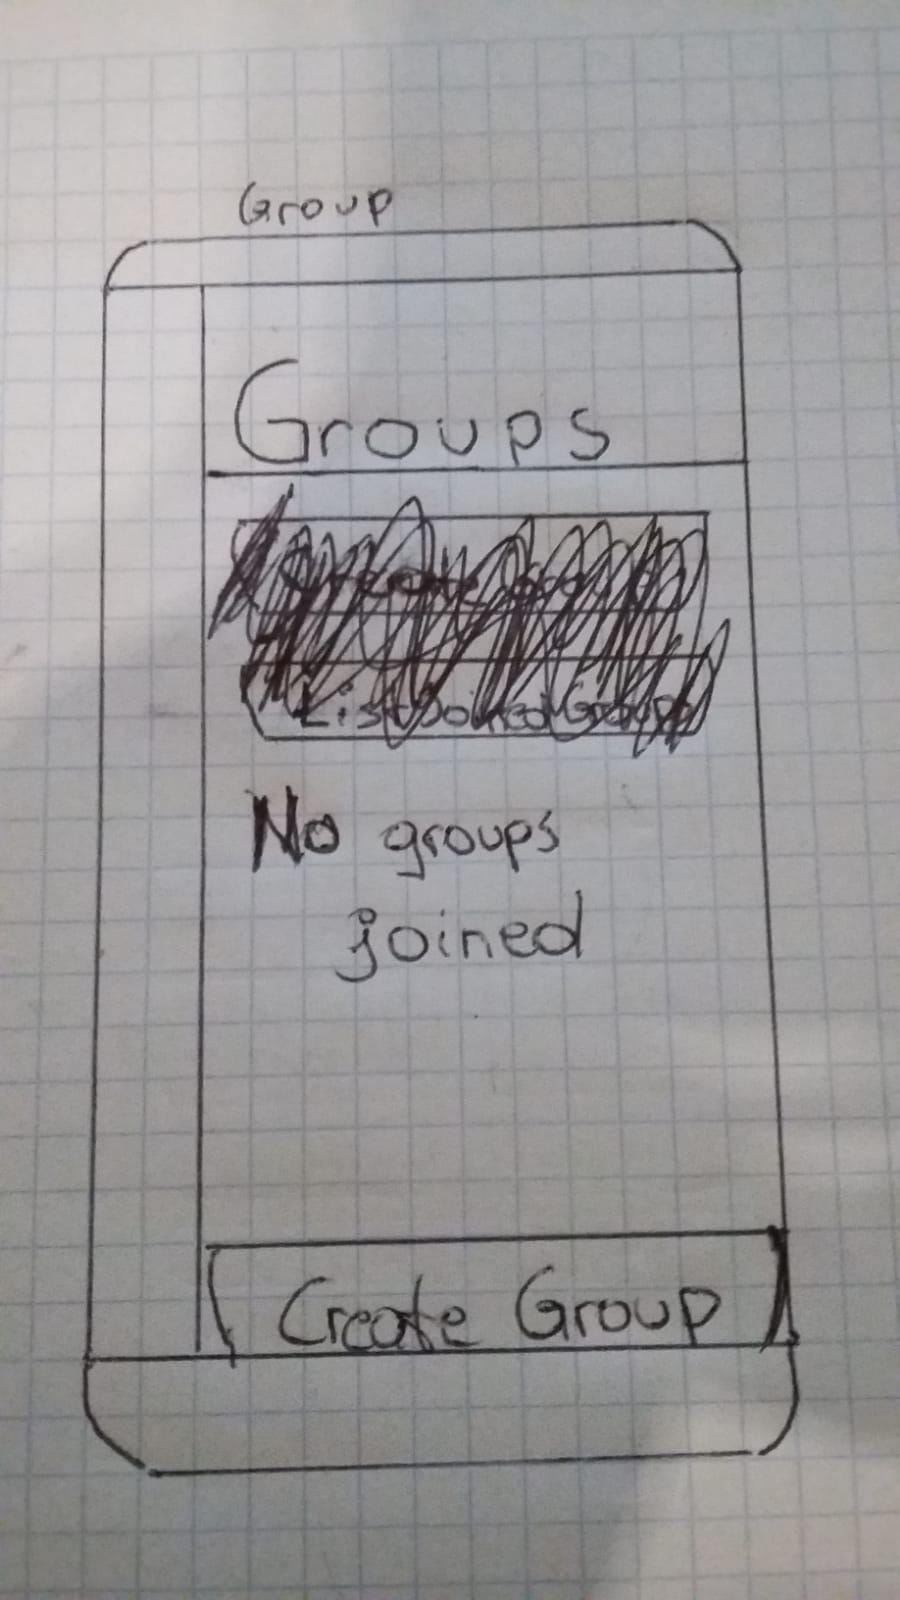
\includegraphics[scale=.2]{Gui/group.jpeg}

\pagebreak


\section{Acceptance Criteria}

\subsection{AC001}

\begin{tabular}{|l|l|}
\hline 
\cellcolor[gray]{0.5}\textcolor{white}{Test step} & \cellcolor[gray]{0.5}\textcolor{white}{Expected behaviour} \\ \hline
Launch an event without declaring & Event wont be created and the user \\ the information which is needed & will be ask to put it in \\ \hline
Inviting the same user twice & Will throw an error which says \\ for the same event & that he cant do that \\ \hline
Inviting an user for an event & Will send him the invitation and notify \\  & the event leader\\ \hline
Change an information of an event & Will notify all participants about \\ & the change \\ \hline
\end{tabular} 

\subsection{AC002}

\begin{tabular}{|l|l|}
\hline 
\cellcolor[gray]{0.5}\textcolor{white}{Test step} & \cellcolor[gray]{0.5}\textcolor{white}{Expected behaviour} \\ \hline
Creating an account with & Sending and error message which tells the \\ missing information & user to fill up the missing information \\ \hline
Joining an event as participat & Getting all the information about the event \\ \hline
Leaving an event as participat & Notyfying the event leader \\ \hline
Removing an participant as & Changing the information \\ event leader & about event \\ \hline
Removing an participant, which & Throwing a error message, which tells the \\ doesn't exist & event leader, that this doesn't exist \\ \hline



\end{tabular}



\pagebreak

\end{document} 